\chapter{Introduction}\label{ch:introduction}

% Audio interactions are becoming ubiquitous in common media platforms, consumer hardware, and immersive technology \citep{yang2019audio}.

\begin{figure}[tbp]
    \centering
    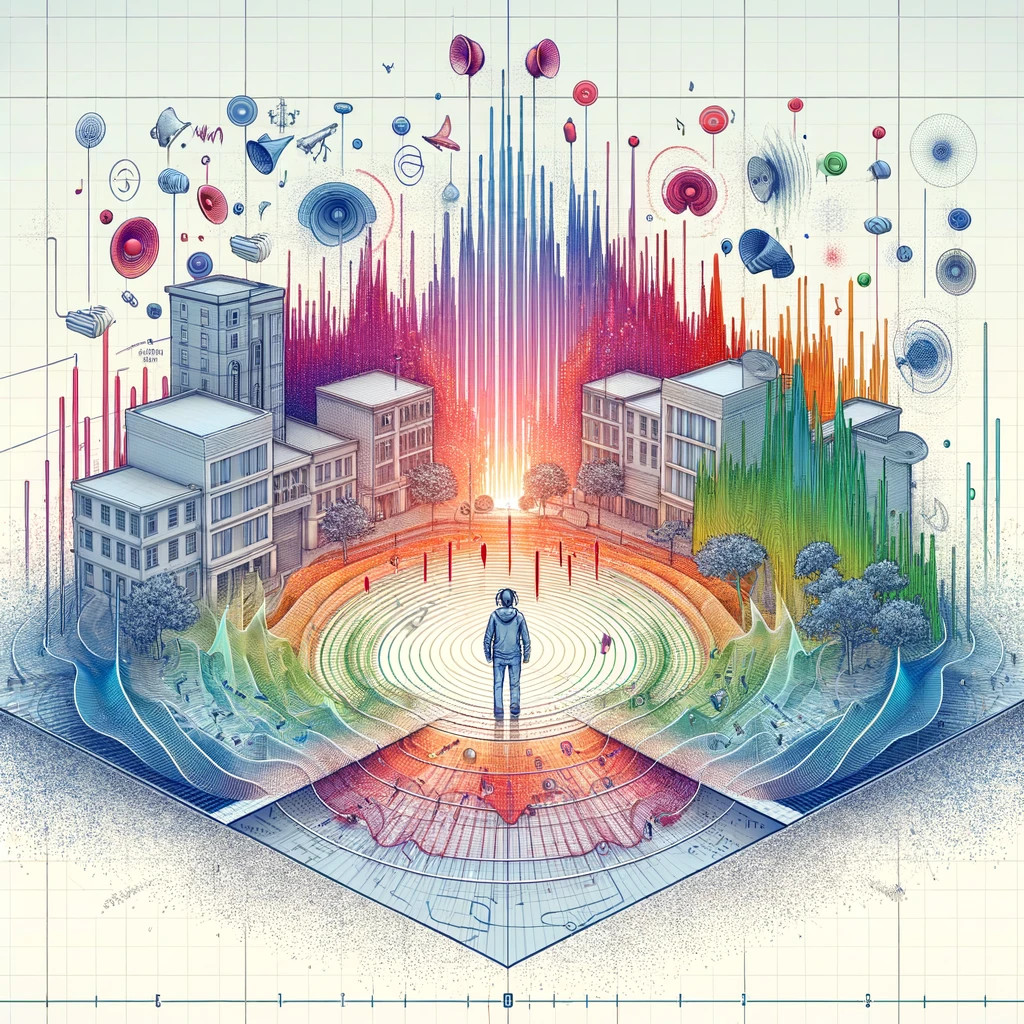
\includegraphics[width=1\linewidth]{thesis_art}
    \caption[Hypothetical virtual environment with a rich soundscape]{A visualisation of a hypothetical virtual environment where a user is immersed in a rich soundscape perceiving many sound-emitting entities. This visualisation is envisioned and produced by the DALL-E text-to-image model (\url{https://openai.com/dall-e-3})}
\end{figure}

Since the first experiments by~\cite{sutherland1968head} in engineering systems to present users with stimuli to convey three-dimensional virtual objects, research domains around immersive virtual environments have only risen in popularity and become central topics in the major journals and scientific venues in computing.\par
\acrfull{ve} constantly improve their ability to express virtual worlds in multimodal platforms \citep{rubio2017immersive}. Their applications range from computer games, including serious and educational games, to digital museums, cultural preservation, and architectural design, raising the need for realistic and compelling representations of \acrshortpl{ve}. Realism is achieved by emulating the physics of the natural world, improving user engagement and performance in tasks in immersive applications. Realism and presence in the audiovisual domains are strongly related to the interaction with scene elements via perception of stimuli \citep{zimmons2003influence, lokki2005navigation}. Sound cues alone, for instance, are sufficient to enable users in \acrshortpl{ve} to pinpoint locations of sound-emitting entities in a scene by using auditory sound localisation, a natural ability associated with the human auditory system.\par
\section{Motivations}
\subsection{Realism and Presence in Immersive Applications}
Creating compelling and realistic auditory displays is problematic, providing many challenges in the acoustics and computer graphics research communities due to the complex nature of sound in the real world. As the acoustic principles that govern how sound propagates in space are difficult to reproduce in digital systems, many methods exist, providing variable orders of approximations, depending on the application. Such approaches emulate the wavefield of an environment, simulating how sound interacts with boundaries and scene objects. A subset of these can reproduce phenomena of sound, such as diffraction, reflection, and refraction, which are determinants of realism as they emulate how waves bend around obstacles. Such phenomena make the simulated wavefield dependent on the accuracy of scene geometry and materials represented in a \acrshort{ve} \citep{kuttruff2016room}.\par
Graphics and visual rendering systems advance towards better methods for representing geometry and objects of an environment, improving the relationship between virtual entities and their expression through multimodal stimuli. Such a relationship determines realism and presence evoked in user interactions when rules of the physical world can be applied to multimodal displays to reason about these virtual entities. \textit{Half Life: Alyx} is an example of a modern game that uses advances in multimodal rendering and interactions to create a complex physics system that allows users to manipulate and leverage the virtual environment reproducing natural, life-like physical interactions \citep{bollmer2022embodied}.
Psychological factors relating to the human perception system determine the degree of realism, presence, and embodiment evoked by multimodal stimuli produced by rendering systems. The perception of virtual entities in a complex virtual scene is ultimately subjective, requiring rendering methods to consider aspects of human perception.

\subsection{Immersion and Realism in Auditory Stimuli}
% intro to audio rendering
Auditory information is paramount to human perception in natural and virtual environments, helping in orientation and navigation, increasing immersion and aiding in task performance \citep{lokki2005navigation, bork2015auditory, shivappa2016efficient}. The sound field a listener perceives is a function of the surrounding environment's shape, dimensions, boundaries, and transmission mediums. Even though the physics of sound propagation makes realistic audio rendering challenging, many proposed approaches allow realistic simulations of sound fields in \acrshort{ve}. Computer games, compelling simulations, and digital tourism benefit from realistic audio rendering and improved auditory presence evoked in virtual environments \citep{lokki2002creating, selmanovic2020vr}.\par
The realism of digital media has increased in recent years thanks to recent advances in computer games technology \citep{rubio2017immersive}. As a listener in a sound transmission, the human auditory system is aware of acoustic characteristics manifesting in auditory cues, which enable spatial hearing abilities, such as sound localisation, aiding interaction tasks with objects in the world. Intrinsic acoustic characteristics are dependent on the sound transmission's wavefield, dictated by structural properties of the environment, associated with boundaries and materials, as they interact with sound propagating to the listener's ears. Acoustic rendering methods simulate real or virtual auditory environments by deriving from sound propagation algorithms that discretise the geometrical representation of an environment to synthesise a wavefield. They render spatialised sound adapting signal processing chains to reproduce realistic sound transmission in the simulated wavefield, considering the listener's position, orientation, and physical characteristics, described by \acrfullpl{hrtf} \citep{hulusic2012acoustic}.\par

\subsection{Modern Immersive Human-Computer Interfaces}
% Intro to Audio in XR
\acrshort{ar} platforms are suited for a range of use cases within areas of training, digital tourism, or games, thanks to the enhanced interactions with the physical world surrounding the user. An \acrshort{ar} platform, which throughout this work defines the set of technologies and hardware interfacing the user with virtual and physical environments via audio-visual and holographic displays, gesture, eye, and body tracking, and with the physical world via computer vision, scene understanding, space reconstruction, and spatial mapping techniques. This broad range of sensing technologies and multimodal interefaces open avenues for addressing tasks within research domains where users interact with entities in \acrshort{ar} space. Accessibility, for instance, is a research domain benefitting from the development of this platform by helping users with disabilities navigate and understand their surrounding scene, leveraging the sensing data provided by the platform and performing speech recognition or scene understanding techniques \citep{mehra2020potential}.\par
The increasing popularity of immersive media proliferating within an increasing number of industry and research domains \citep{park2022metaverse}, enabling HMDs to support applications ranging from training scenarios, education, social learning, operation learning \citep{harris2020effect, ahir2020application} to entertainment or gaming \citep{yuen2011augmented, ke2018virtual} or to digital tourism and cultural preservation use cases \citep{schofield2018viking, selmanovic2020cultural}. \acrshort{ar} applications in modern HMDs, e.g. the Microsoft Hololens 2\footnote{\url{https://www.microsoft.com/en-gb/hololens}\label{note:ms-hl2}}, can provide real-time space reconstruction, spatial mapping, and scene understanding features\footnote{\url{https://learn.microsoft.com/en-us/hololens/hololens2-hardware}\label{note:ms-hl2-hw}}. Such features have unlocked crucial potential in the sound rendering subdomain, as emerging novel pipelines allow acoustic simulation techniques to be deployed to \acrshort{ar} HMDs, as discussed in Chapter~\ref{ch:ar-pipeline}. As a result, users experiencing holographic content projected onto their surroundings can perceive realistic sound propagation from holograms. Experiencing realistic sound rendering in \acrshort{ar} directly impacts the above-mentioned industry domains and research as HMDs become more ubiquitous and accessible.\par
These example applications and use cases of \acrshort{ar} with modern HMDs rely on auditory stimuli for conducting activities or completing tasks in VEs, such as navigation, locomotion, or entity localisation. As discussed in Chapter~\ref{ch:Background}, the hearing sense relies on acoustic information encoded in auditory stimuli to predict or triangulate the position of sound-emitting objects within the hearing range.

% general field 
\subsection{Limiting Factors of Immersive Technology within Audio Interfaces}
% TODO: Merge the two together
The current state of \acrshort{ar} allows auditory interactions between virtual entities projected around the user. These are possible thanks to the advances in game engines, enabling the construction of complex immersive scenes that can be experienced through \acrshortpl{hmd}. The field of \acrfull{aar}, as defined by~\cite{yang2022audio} and~\cite{yang2019audio} advances towards realistic auditory interactions, allowing for context-aware stimuli and reflecting the behaviour of sound transmissions in the physical world.\par
Current frameworks available to build complex augmented scenes, such as the Microsoft Mixed Reality Toolkit\footnote{\url{https://learn.microsoft.com/en-us/windows/mixed-reality/develop/unity/unity-development-overview}}, provide a limited suite of tools to implement audio sources, beyond basic spatialisation effects. For instance, audio emitted from virtual sound sources projected onto the real world does not consider basic principles of acoustics.\par
One cause is due to the complexity around the process of simulating sound propagation effects in dynamic virtual environments. Despite, decades of research advancing the field of sound rendering, computing acoustic effects in real-time is a difficult and expensive task. The ever-changing surroundings and the limited onboard compute availability in \acrshortpl{hmd} pose additional challenges to the task.
These limitations prevent users from experiencing realistic \acrshort{ar} sounds as they cannot exploit natural phenomena to perform tasks associated with sound perception. Based on factors of sound transmissions from a sound-emitting entity to the two ears. Sound localisation, as an example, is a natural ability that humans perform with everyday sounds where they pinpoint the location of an object by its propagated audio. Realistic sound rendering techniques can allow listeners to apply psychoacoustic abilities like sound localisation in sound transmissions within virtual environments or augmented environments. These use representations of real or virtual space to create an approximated acoustic model where sound propagation can occur, taking into account the architectural and physical characteristics of the environment. Hence, the spatial mapping and scene understanding capabilities of \acrshort{ar} \acrshort{hmd} can provide sound rendering techniques with real-time geometry and acoustic features associated with the users' surroundings, which are needed for realistic sound propagation.\par
% our system 
On the one hand, there is a large body of research in psychoacoustic abilities such as localisation or clustering \citep{lee2011relationship} generating recommendations for audio reproduction apparatus; and on the other hand, there are emerging pipelines allowing customisable binaural rendering for immersive technology, making it possible to encode acoustic phenomena in audio stimuli to match visual stimuli \citep{plinge2018six}. There is a lack of research towards combining the two research domains in emerging areas of \acrshort{ar}, exploring the potential in the relationship between the physical space surrounding the user and auditory interactions. The experiment will ask human participants to perform tasks requiring them to experience sound transmissions in \acrshort{ar} and conduct tasks dependent on psychoacoustic abilities. The study will measure and gather data on the performance of participants conducting tasks to compare realistic sound propagation against current sound rendering methods.\par

\section{Significance}
A novel aspect of the proposed work is the application of computer vision methods to infer acoustic data associated with materials and boundaries in environments to enable sound rendering systems such as acoustic simulation methods, to adapt to unseen complex scenes in materials.
% Potential contributions of this novelty include Augmented Reality (AR) applications \citep{liu2018technical}, where users can control interactions between virtual objects and the real world. A possible outcome from the proposed work would allow AR applications to render sounds emitted from virtual objects considering acoustic aspects of real environments. \par
Contributions deriving from this work would feed into computer games technology applied to entertainment, serious games, architectural acoustics, and digital tourism. Architectural acoustic applications would benefit from automated reconstructions of auditory spaces from real environments, allowing designers to create and test acoustic models with \acrshort{ar} applications or game engines \citep{berardi2016acoustic}. Digital tourism, besides, would benefit from improvements in sound rendering pipelines to let users experience and interact with reconstructions of places of cultural interest \citep{schofield2018viking}.\par
The need for realistic audio in computer games is of growing importance as it allows players to immerse in virtual worlds. Spatialising sound in three-dimensional worlds, reflecting acoustic features of space, improves the performance of tasks associated with auditory cues, enhancing the overall experience and quality of games. 
Activities in virtual environments using auditory cues, such as navigation in space and sound localisation are fundamental in simulations and training applications \citep{lokki2005navigation}. Hence, sound rendering systems are of crucial importance in these fields.

\section{Research Aim}
\begin{figure}[htbp]
    \centering
    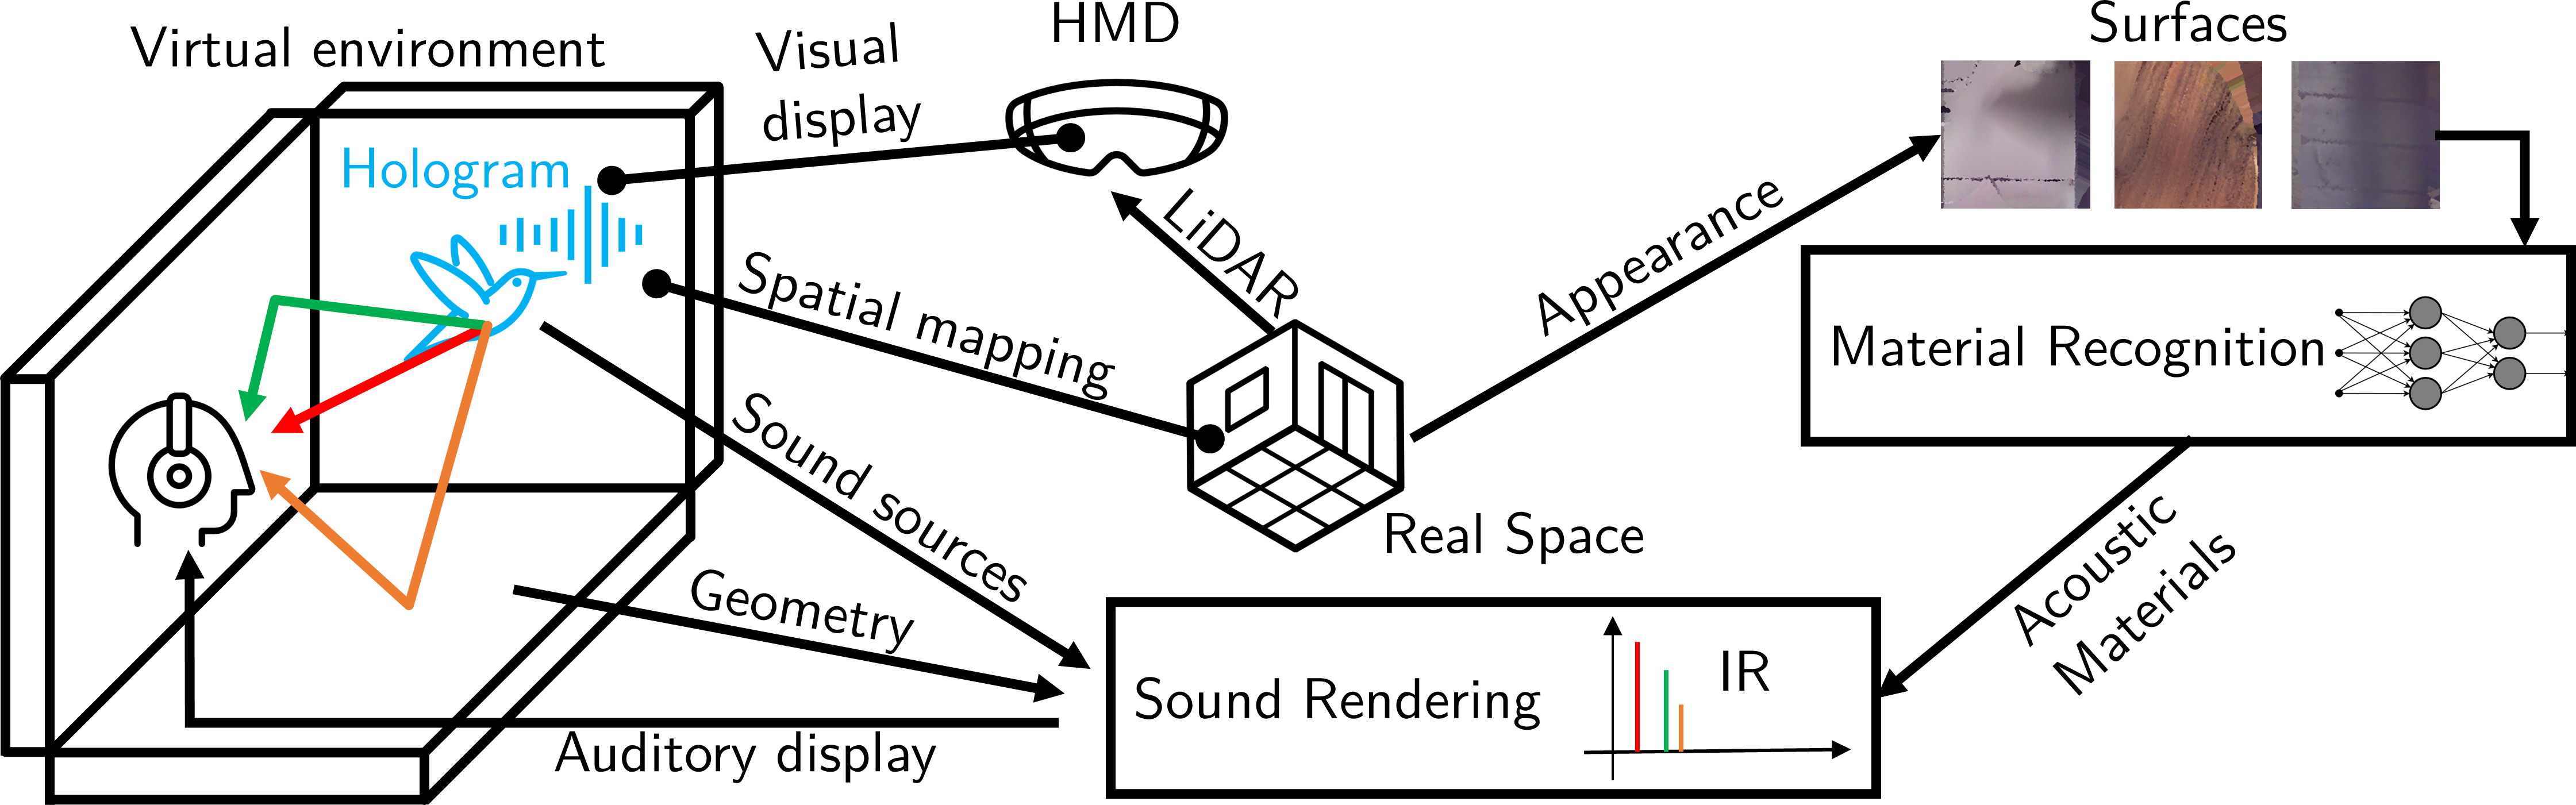
\includegraphics[width=1\linewidth]{phd_functional_diagram}
    \caption[Proposed pipeline schematic overview]{Overview of the interactive acoustic rendering system for \acrshort{ar} proposed as part of the thesis work.}
    \label{fig:proposed-system-diagram}
\end{figure}
The proposed work aims to explore rendering pipelines with respect to sound propagation in VEs, studying the relationship between the perceived wavefield and the environment’s visual representation: materials, structural geometry, and physical characteristics of objects in complex scenes.


\section{Objectives}\label{sec:thesis-objectives}
\begin{itemize}
    \item To review the current state of audio rendering in virtual environments, assessing their limitations, realism and computational requirements to investigate their applications in real-time acoustic simulations for complex scenes.
    \item To explore how, in modern approaches to acoustic simulations, visual representations of materials relate to simulated soundfields.
    \item To design and test systems to automatically attribute acoustic materials to scene geometry in virtual environments, recognising and distinguishing between materials in the acoustic and visual domains.
    \item To study and evaluate the application of sound rendering methods with acoustic material recognition.
    \item To design and propose a novel pipeline for acoustic rendering applied to augmented reality platforms.
    \item To investigate psychoacoustic and human factors in auditory displays created by the proposed pipeline by testing an augmented reality prototype.
\end{itemize}

\section{Thesis Structure}

\begin{figure}[htbp]
    \centering
    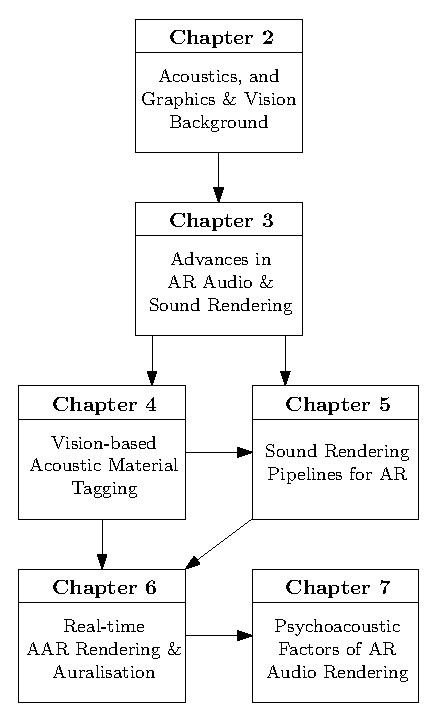
\includegraphics[width=0.6\linewidth]{thesis-structure}
    \caption[Thesis structure overview]{Structure and dependency graph of Chapters of this thesis. Introductory and conclusive Chapter~\ref{ch:introduction} and~\ref{ch:Conclusion}, respectively, were omitted for simplicity.}
    \label{fig:thesis-structure}
\end{figure}

\section{Chapter List}
\textbf{Chapter~\ref{ch:introduction}} \textit{Introduction} presents the goal and objectives to the reader, starting from the rationale and factors motivating this research, providing background on research domains of interest, and illustrating the contributions and how these are structured throughout the Chapters.

\textbf{Chapter~\ref{ch:Background}} \textit{Background Research} provides the reader with foundations on wave physics, sound propagation, acoustic data in digital systems, as well as computer graphics in the context of handling and representing virtual environments. The reader is also introduced to elements of machine learning to provide grounding for vision-based scene understanding systems designed as part of the thesis aim.

\textbf{Chapter~\ref{ch:litReview}} \textit{Advances in Visual-Acoustic Mapping and Sound Rendering Pipelines} reports relevant bodies of literature relevant to research and industry domains overlapped by the proposed overarching system. Limitations of the current state of industry and research on these domains are reviewed alongside visions and research directions identified by authors, defining the contributions discussed across the thesis.

\textbf{Chapter~\ref{ch:Materials}} \textit{Methods for Acoustic Characteristics Retrieval from Complex Virtual Environments} introduces the design and application of computer vision methods for extracting acoustic characteristics from virtual environments, which constitute building blocks for the proposed pipeline and address acoustic material tagging, a crucial problem in the domain of sound propagation for virtual environments.

\textbf{Chapter~\ref{ch:acousticrendering}} \textit{Geometrical Acoustics Rendering Pipelines for Augmented Acoustics} integrates acoustic material tagging systems with standard acoustic rendering techniques based on approximating acoustic waves with geometrical primitives. This Chapter aims to provide a baseline acoustic renderer for designing the interactive AR pipeline proposed in the following Chapter.

\textbf{Chapter~\ref{ch:ar-pipeline}} \textit{Towards Scene-Aware Acoustic Rendering Pipelines for Augmented Audio Reality} demonstrates the design of the proposed pipeline, expressed by the overarching research aim, as an end-to-end system for Augmented Reality Head-Mounted Displays, illustrating technical components and workflows for achieving real-time interactions. Considering related work reviewed by Chapter~\ref{ch:litReview}, visions, impact, and future research are discussed, indicating avenues for expansions.

\textbf{Chapter~\ref{ch:ar-pipeline}} \textit{Psychoacoustic Characterisation of Rendering Pipelines for Augmented Acoustics} deploys a prototype to an augmented reality platform in order to conduct a set of psychoacoustic tests on the pipeline illustrated by the previous Chapter. Here, a novel methodology and framework for testing the characterisation of sound rendering pipelines are evaluated and discussed.

\textbf{Chapter~\ref{ch:Conclusion}} \textit{Conclusions} provides a high-level discussion on the results gathered from objective and subjective experiments gathered by testing components of the proposed system, reflecting on broader impact, detailing potential use cases, and recommending future expansion avenues.

\section{Contributions}
The main contributions of this thesis are the proposal, design, prototyping, and testing of a novel pipeline for generating realistic auditory displays in augmented reality platforms, leveraging the potential that modern hardware for holographic rendering has unveiled over the last decades. These contributions represent a stepping stone towards realistic and physically-based auditory interactions in immersive applications, allowing users to understand, reason, and act within a virtual environment from acoustic information conveyed by the augmented reality platform.
These contributions stem from components of the pipeline developed and tested, addressing research questions associated with the design of an end-to-end system. Chapters~\ref{ch:Materials},~\ref{ch:acousticrendering}, and~\ref{ch:Evaluation} present novel systems to address such research questions adopting bespoke methodologies and evaluations. The following list briefly summarises the contributions of this work:
\begin{itemize}
    \item a novel pipeline for realistic acoustic displays for augmented reality platforms;
    \item two novel systems for retrieving acoustic characteristics from virtual environments;
    \item novel testing methodologies for evaluating system for acoustic characteristics retrieval, comparing simulated against real soundfields;
    \item two sound rendering systems integrating methods for acoustic characteristics retrieval;
    \item a study evaluating the proposed sound rendering methods;
    \item a perceptual evaluation investigating psychoacoustic factors of a prototype of the proposed system.
\end{itemize}

The following papers have been published as part of the thesis work:

\begin{enumerate}
    \item Colombo, M., Dolhasz, A. and Harvey, C., 2020, August. A computer vision-inspired automatic acoustic material tagging system for virtual environments. In 2020 IEEE Conference on Games (CoG) (pp. 736--739). IEEE.
    \item Colombo, M., Dolhasz, A. and Harvey, C., 2021, May. A texture superpixel approach to semantic material classification for acoustic geometry tagging. In Extended Abstracts of the 2021 CHI Conference on Human Factors in Computing Systems (pp. 1--7).
    \item Colombo, M., 2021, October. Vision-based acoustic information retrieval for interactive sound rendering. In 2021 IEEE International Symposium on Mixed and Augmented Reality Adjunct (ISMAR-Adjunct) (pp. 487--490). IEEE;
    \item Colombo, M., Dolhasz, A., Hockman, J. and Harvey, C., 2022, August. Acoustic rendering based on geometry reduction and acoustic material classification. In 2022 IEEE Conference on Games (CoG) (pp. 409--416). IEEE.
    \item Colombo, M., Frutos M., Harvey, C., 2024. Psychoacoustic Characterisation of Geometrical Acoustics-based Rendering Pipelines in Augmented Reality. In Review.
    \item Harvey, C., Colombo, M., West, B., Happa, J., and Ali-MacLachlan, I., 2024, October. Immersive Acoustics in Cultural Heritage Applications in Interactive Media for Cultural Heritage. Nicosia, Cyprus: Springer Cham. Book Chapter. In Press.
\end{enumerate}


% \fullcite{colombo2021texture}